% Chapter Template

\chapter{Theory} % Main chapter title

\label{Chapter2} % Change X to a consecutive number; for referencing this chapter elsewhere, use \ref{ChapterX}

In Here we will discus some important facts to get a complete understanding 
in the physical phenomena that is happening. Specially we will develop the 
notions that are crucial in the understanding of the Two-photon imaging using entangled light, been this said 
we will start talking about correlations.

\section{Correlations between two photons}

The term "correlation" is crucial at this point, and it refers to the relation of two or more situations have. For example 
we can establish a correlations between the US dolar currency exchange rate and the prices of technology in one country. These two things have direct relation, if one blows up, the other one will too.
These two situations, or variables, can have a strong correlations or a week one. \\

Indeed in quantum physics we can have a pair of photons that are so strongly correlated, in their possible variables (spatial and temporal),
that we say they are entangled. This statment can leads us 
to a dense discussion about the nature of this entanglement, 
a discussion that were started between Einstein and Bohr in the first years of quantum physics \cite{einstein}.\\

To avoid this discussion we will just talk about correlations, 
and when referring about a pair of correlated photons, we will mean that 
this pair of photons are correlated in one or varius of their variables. 
They can be correlated in momentum, meaning that when one photon have a given $\vec{q}_i$ momentum 
and the other photon have a $\vec{q}_j$ momentum that is determined by the first, this relations is the momentum correlations a we can work out an expression for this relationship.
\subsection{SPDC}

As the title of this work implies, we need a source light that produces pair of photons, 
and we would like to exploit the advantages of strong correlations between them.
The photons generated via spontaneous parametric down conversion (SPDC) are
widely used in quantum optics experiments. The popularity of this source of paired
photons is strongly related to the relative simplicity of its experimental
realisation, and to the variety of quantum features that down converted photons can exhibit. 
The generated photons via SPDC can be correlated in different degrees of freedom, for example 
in polarisation, in frequency and in the equivalent degrees of freedom: 
'orbital angular momentum, space and transverse momentum \cite{spatiocorrelations}.\\

\begin{figure}[h!]
\centering
\label{fig:spdcSimple}
 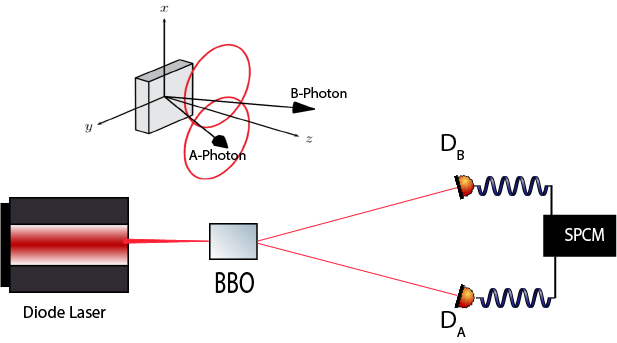
\includegraphics[width=0.65\textwidth]{Figures/spdcSimple.png}
 \caption{Simple Experimental setup for the SPDC process} 
\end{figure}


SPDC is an optical process in which focus a beam pump, that is 
propagating in the $z$-direction, to a nonlinear crystal of length $L$. Using first order perturbation 
and the paraxial approximation, the two-photon state is given by:
\begin{equation}
\label{eq:stateFunComplex}
\ket{\Psi}=\int dq_B dq_A d\Omega_B d\Omega_A 
\text{x} [\Phi(q_B,\Omega_B;q_A,\Omega_A) \hat{a}^{\dagger} (\Omega_B,q_B) \hat{a}^{\dagger}(\Omega_A,q_A) \\
+ \Phi(q_A,\Omega_A;q_B,\Omega_B) \hat{a}^{\dagger}(\Omega_B,q_B) \hat{a}^{\dagger}(\Omega_A,q_A)]   \ket{0}  
\end{equation}
Where this state function depends on the transverse wave vectors $q_n=(q_n^x,q_n^y)$ and frequency detuning, $\Omega_n=\omega_n-\omega_0^n$, 
around the central frequencies, $\omega_0^n$, for the photon at the path $A$ or $B$ ($n=A,B$).
The $\Phi(q_B,\Omega_B;q_A,\Omega_A)$ and $\Phi(q_A,\Omega_A;q_B,\Omega_B)$
are the mode functions or biphotons that contains all the informations about the correlations
between the pair of down-converted photons. The operator $\hat{a}^{\dagger}$ indicates the creations of an $n$-polarized photon with transverse momentum $q_n$, 
and frequency detuning $\Omega_n$ \cite{physicsGhost}. \\

In the optical table we put a polariser at certain directions at the detections modules,
filtering some of the photons before reaching the detector, this filtering also have a mathematical effect in our model, 
it is posible now to write \ref{eq:stateFunComplex} different, dropping one term:
\begin{equation}
\label{eq:stateFun}
\ket{\Psi}=\int dq_B dq_A d\Omega_B d\Omega_A 
\text{x} [\Phi(q_B,\Omega_B;q_A,\Omega_A) \hat{a}^{\dagger} (\Omega_B,q_B) \hat{a}^{\dagger}(\Omega_A,q_A) 
] \ket{0}  
\end{equation}

The mode function  $\Phi(q_B,\Omega_B;q_A,\Omega_A)$ is related with the joint probability of detecting both an $B$-polarized
photon, with tranverse momentum $q_B$ and frequency detuning $\Omega_B$, at the detector $B$ 
and an $A$-polarized
photon, with tranverse momentum $q_A$ and frequency detuning $\Omega_A$, at the detector $A$. 

\subsubsection{Phase matching conditions}
In particular, $\Phi(q_B,\Omega_B;q_A,\Omega_A)$ reads \cite{spatiocorrelations}:
\begin{equation}
\label{eq:mode}
\Phi(q_B,\Omega_B;q_A,\Omega_A) = \mathcal{N} \alpha(\Delta_0,\Delta_1) \beta(\Omega_B,\Omega_A) \text{ x }
sinc \left( \frac{\Delta_k L}{2} \right) e^{i \frac{\Delta_k L}{2}}
\end{equation}
Where $\mathcal{N}$ is a normalisation constant, $\alpha(\Delta_0,\Delta_1)$
and $\beta(\Omega_B,\Omega_A)$yields the informations of the pump's transverse 
and spectral distribution, respectively, L is the length of the nonlinear crystal.
For the process that is happening inside the crystal, there are some conditions that have to be fulfilled. These conditions are related with the energy and momentum conservations inside the parametric down conversion process.
The terms $\Delta_0$, $\Delta_1$ and $\Delta_k$ are functions that result from the phase matching conditions and read:
\begin{equation}
\Delta_0=q_B^x + q_A^x
\end{equation}
\begin{equation}
\Delta_1= q_A^y cos\phi_A + q_B^y cos\phi_B - N_B \Omega_B sin\phi_B + N_A \Omega_A sin\phi_A - \rho_B q_B^x sin\phi_B 
\end{equation}
\begin{equation}
\Delta_k=N_p(\Omega_B+\Omega_A)-N_B\Omega_B cos\phi_B - N_A\Omega_A cos\phi_A -q_B^y sin\Omega_B + q_A^y sin\Omega_A + \rho_p \Delta_0 - \rho_B q_B^x cos\phi_B
\end{equation}
The angles $\phi_B$ and $\phi_A$ are the creation angles of the down-
converted photons inside the crystal with respect to the pump’s
propagation direction, whereas the angles $\rho_p$ and $\rho_B$ account for
the walk-off of the pump $p$ and the $B$ down-
converted photon, respectively. 
In this study, $\phi_B$ and $\phi_A$ are treated as constants, 
mainly because the scanned transverse momentum regions represent a small portion around
the emission angles. $N_n$ denotes the inverse of the group velocity for each photon.



\subsection{Spatial Correlations}

In order to observe the correlations presented in \ref{eq:mode} we have to take into account some considerations about the descrption of the things we have in optical table.
First of all we have a pump beam with a Gaussian profile with waist $w_p$ 
in such way that $\alpha (\Delta_0,\Delta_1 ) \propto \text{exp}[-w_p^2 (\Delta_0^2 + \Delta_1^2 )/4]$, a CW pump laser, mathematically represented by
$\beta (\Omega_B , \Omega_A) \propto \delta(\Omega_B + \Omega_A)$. Making the aproximations for the sinc function by a Gaussian fuctions with the same width at $1/e^2$ of its maximum,
i.e., $sinc(x) \approx \text{exp}(-\gamma x^2)$ with $\gamma$ equal $0.193$.
The mode function reduces to:

\begin{equation}
\label{eq:modeSim}
\Phi(q_B,\Omega_B;q_A,\Omega_A) = \mathcal{N} \beta (\Omega_B , \Omega_A)
\text{ x exp}\left[ -\frac{w_p^2 (\Delta_0^2 + \Delta_1^2 )}{4}-\gamma \left(\frac{\Delta_k L}{2} \right)^2 + i\frac{\Delta_k L}{2} \right]  
\end{equation}

In order to observe the transverse correlations (spatial correlations), the 
frequency information has to be traced out, in the optical table this can
be achieved by placing some interferometer filters before detection. This spectral
filters are modeled as $f_n (\Omega_n)=\text{exp}[-\Omega_n^2/(4\sigma_n^2)]$, with bandwidth $\sigma_n$ chosen to achive a regimen where the 
spatial-spectral correlations are completely broken \cite{broke}. 
To achieve this mathematically we have to integrate \ref{eq:modeSim} around the
spatial variables:
\begin{equation}
\label{eq:modeSpa}
\tilde{\Phi}(q_B,q_A) = \int d\Omega_B d\Omega_A f_B(\Omega_B)f_A(\Omega_A) \Phi(q_B,\Omega_B;q_A,\Omega_A)
\end{equation}

\begin{figure}[h!]
\centering
{  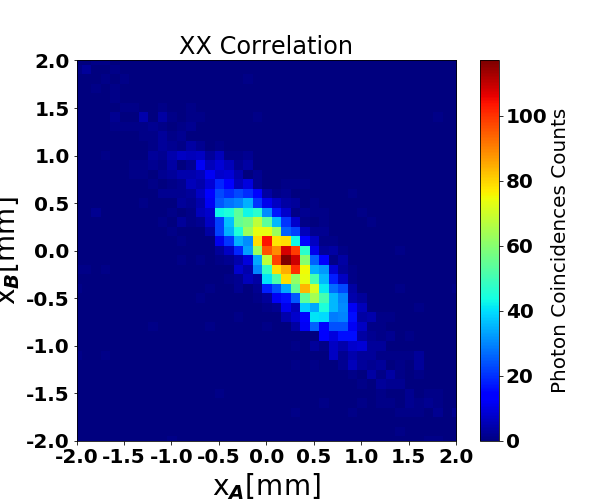
\includegraphics[width=0.48\textwidth]{Figures/xxCorrelation.png} }
{  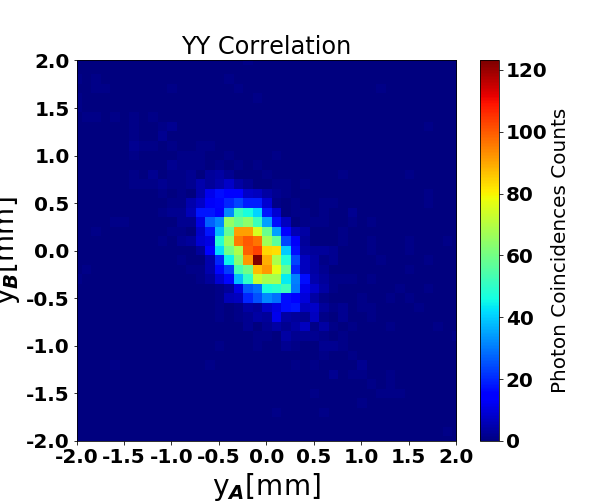
\includegraphics[width=0.48\textwidth]{Figures/yyCorrelation.png} }
\caption{Experimental Spatial correlations between a pair of down-converted photons. Right image shows the correlation in the x variable. Left shows the correlation in the y variable, Beam propagating in the z direction}
 \label{fig:corre}
\end{figure}
Figure \ref{fig:corre} show a couple of examples of how these correlations we are talking about look like. These correlations have some king of circular shape,
and show how strong is the posibility of detecting a photon at a given position, looking at the first graph, there is a great chance
of detecting simultaneously a photon at $x_B=0$ and at $x_A=0$. Now if we look at the left graph, it is showing the correlation 
of the pair of photons in the $y$ direction, there is a significant probability of measuring simultaneously a photon at $y_B=0.4$ 
and at $y_A=-0.4$. It is interesting how in this case there is a "negative" correlation, the expected position at which we will find the other photon, is at the same, but negative position.
Another interesting fact we have to point out, is that this correlations algo can be sharper, the x correlation have a more circular shape, making wider the posible values for a given $x_B$. In contrast the y correlation is more eliptic, meaning it restring the posible values por a given $y_B$.
It is easy to think how a strong correlation should look like, a strong correlations in spatial variables would mean that if we have the position of one photon at the position $x_B$ we immediately would know which $x_A$ have the other photon, this king of ideal spatial correlation would look like a straigth line
really thin, Figure \ref{fig:idealCorre}. 


\begin{figure}[h!]
\centering
{  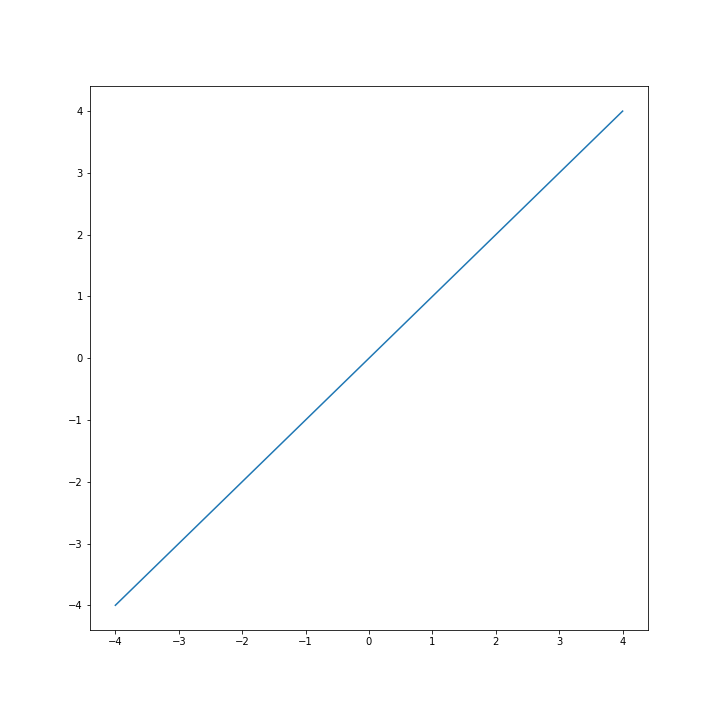
\includegraphics[width=0.48\textwidth]{Figures/idealPositiveCorrelation.png} }
{  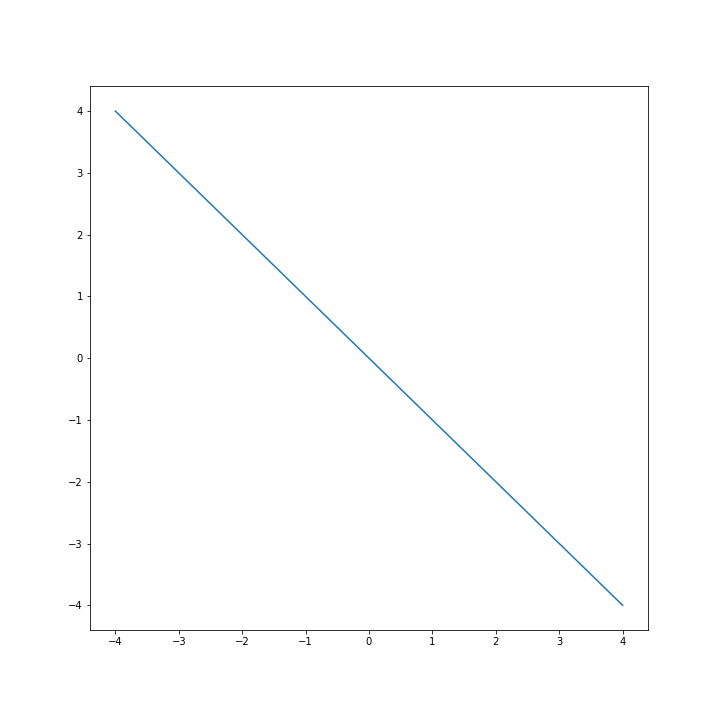
\includegraphics[width=0.48\textwidth]{Figures/idealNegativeCorrelation.png} }
\caption{Positive(right) and Negative(left) ideal spatial correlations}
 \label{fig:idealCorre}
\end{figure}


\subsection{Tunable Spatial Correlation SPDC source light}
It is clear that both \ref{eq:modeSim} and \ref{eq:modeSpa} depend on $w_p$, the pump waist. If we change this 
parameter and keep the rest of the parameters constant, the term in the exponential function $[-w_p^2 (\Delta_0^2 + \Delta_1^2 )/4]$ will variate,
making changes in the shape of the original mode function. As it was mentioned here before and in \cite{omar}, the mode function
contains all the informations about the correlations of the generated down converted photons. Hence changing the pump waist $w_p$
will change the correlations of the generated pair of photons.




\section{Imaging}

Assuming we have an object that have its own light or its externally illuminated,
imaging means collecting that light that is emitted from the object. Each point
of the surface of the object will emit spherical waves to all possible directions,
being this said, What is the probability to have a spherical wave collapsing into a point or small spot? 
Obviously, the chance is practically zero unless an imaging system is applied.
\\
The concept of optical imaging was well developed in classical optics and the Figure
\ref{fig:imaging} schematically illustrates a standar imaging setup. In this setup 
an object is illuminated by a radiation source, an imaging lens is used 
to focus the scattered and reflected light from the object onto an image plane 
which is defined by the “Gaussian thin lens equation”\cite{hecht}:
\begin{equation}
\frac{1}{S_0}+\frac{1}{S_i}=\frac{1}{f}
\end{equation}
 where $S_0$ is the distance between the object and the imaging lens, $S_i$ the distance 
between the imaging lens and the image plane, and $f$ the focal lenght of the imaging lens. This equation defines
a point-to-point relationship between the object plane and the image plane: any radiation starting from a point on the object will colapse at a certain point at the image plane.
\\
\begin{figure}[h!]
\centering
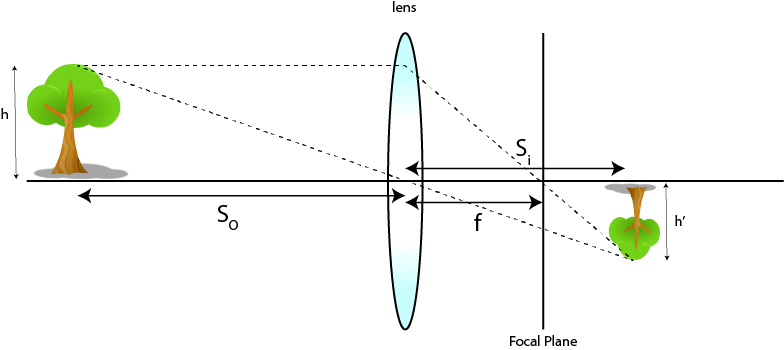
\includegraphics[width=0.6\textwidth]{Figures/imaging.png}
\caption{Optical imaging: a lens produces an image on an object at $S_i$. This distance is defined
by the Gaussian thin-lens equation} 
\label{fig:imaging}
\end{figure}
This one-to-one correspondence in the image-forming relationship between the object and the image planes produces a perfect image.
The observed image can be magnified or demagnified, for example, in the 
Figure \ref{fig:imaging} the original object is a tree, and it is demagnified at the image plane. This depends on which optical 
system are we using, what kind on lenses are involved and the distance between object and them.

\subsection{Standar Imaging}

The observed image is a reproduction of the illuminated object, mathematically
corresponding to a convolution between the object distribution fuction $ |T(\vec{\rho_o})|^2$ (aperture function) 
and a $\delta$-function, which is present for the perfect
point-to-point correspondence \cite{introquantumoptics}:
\begin{equation}
I(\vec{\rho_i})=\int_{obj} d\vec{\rho_o} |T(\vec{\rho_o})|^2 \delta(\vec{\rho_o}+\frac{\vec{\rho_i}}{m})
\end{equation}
where $I(\vec{\rho_i})$ is the intensity at the image plane, $\vec{\rho_o}$ and $\vec{\rho_i}$ are 2-D vectors of the
transverse coordinates in the object and image planes, respectively, and
$m=s_i/s_o$ is the image magnification factor.

In reality, we are limited by the finite size of the optical system, we may never obtain a perfect image.
we have to take into account the constructive-destructive interference present
in this phenomena, because of the wave nature of light. The point-to-point correspondence turns into a point-to-"spot" relationship.
For further informations about this "real life" situation check the \ref{appendix:intensity}.



\subsection{Two-photon Imaging}

Two-photon imaging consist after all, in reconstructing an image of an object. But in this case we use two dectector located in diferents paths of the light. By using the dectections of them separately we get a constant signal, with no information about the object, Figure \ref{fig:twoPhotonSetup}. But if instead we use the signal of them both, counting conincidences, we can reconstruct the double slit in Figure \ref{fig:twoPhotonSetup}. \\


\begin{figure}[h]
\centering
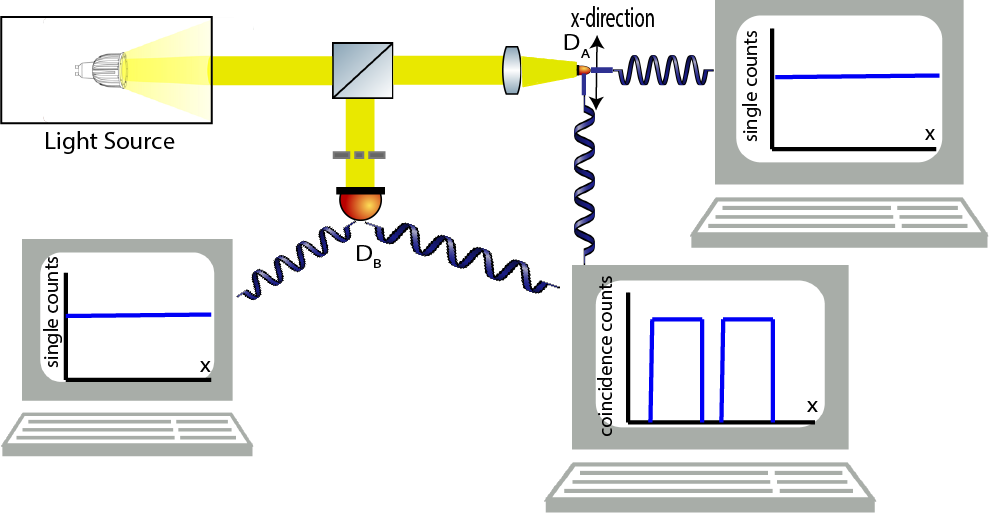
\includegraphics[width=0.7\textwidth]{Figures/twoPhotonSetup.png}
\caption{Simple schematic for the Two-photon Imaging} 
\label{fig:twoPhotonSetup}
\end{figure}
In order to reconstruct the image of the double slit, we have to introduce some kind of spatial dependence, the object, in this case the double slit, is distributed along a transverse direction of the light propagation. But what we have learnt is that scanning along the x-direction (asuming that light propagates along the z-direction), in the path that have no interaction with the object $D_2$, and colecting all the light that interacts with the object $D_1$, gathering no spatial information. We reconstruct the double slit in the coincidences counts, every time we have a photon detected going througt the double slit, and a photon at a certaint position $x_i$, we graph coincidences vs ${ x_i }$ and we get the image of the double slit, Figure \ref{fig:twoPhotonSetup}. 


The optical imaging used the photons at the image plane, to form the image. In other 
words it takes measure one photon per spot at the image plane. For the type-one and type-two
two-photon imaging, in certain aspects the behaviour is similar as that of the classical.
They both exhibit a similar point-to-point imaging-forming function, except the 
two-photon image is only reproducible in the joint-detection between two independent photodetectors,
and the point-to-point imaging-forming function is in the form of second-order correlation,
\begin{equation}
R_{12}(\vec{\rho_i})=\int_{obj} d\vec{\rho_o} |T(\vec{\rho_o})|^2 G^{(2)}(\vec{\rho_o},\vec{\rho_i})
\end{equation}
where $R_{12}(\vec{\rho_i})$ is the joint-detection counting rate between photodetectors $D_1$ and $D_2$.
$G^{(2)}(\vec{\rho_o},\vec{\rho_i})$ is a nontrivial point-to-point second-order correlation
function, corresponding to the probability of observing a joint photo-detection event
at the coordinates $\vec{\rho_o}$ and $\vec{\rho_i}$. The physics behing $G^{(2)}(\vec{\rho_o},\vec{\rho_i})$
is what changes between type-one and type-two two-photon imaging.

%----------------------------------------------------------------------------------------
%	SECTION 1
%----------------------------------------------------------------------------------------
\subsubsection{Two-photon Imaging using entangled photon}

In the previous section we introduced the notion of two-photon imaging , but we didn't care much about the nature of the source light. For this case we will use entangled photon as the source light, we will separate the pair of entangled photons by means of a polarization beamspliter. The first type-one two-photon imaging experiment was demonstrated by Pittman in 1995\cite{pittman}. The schematic setup of the experiment is shown in the Figure \ref{fig:pittman}. \\ 

\begin{figure}[h]
\centering
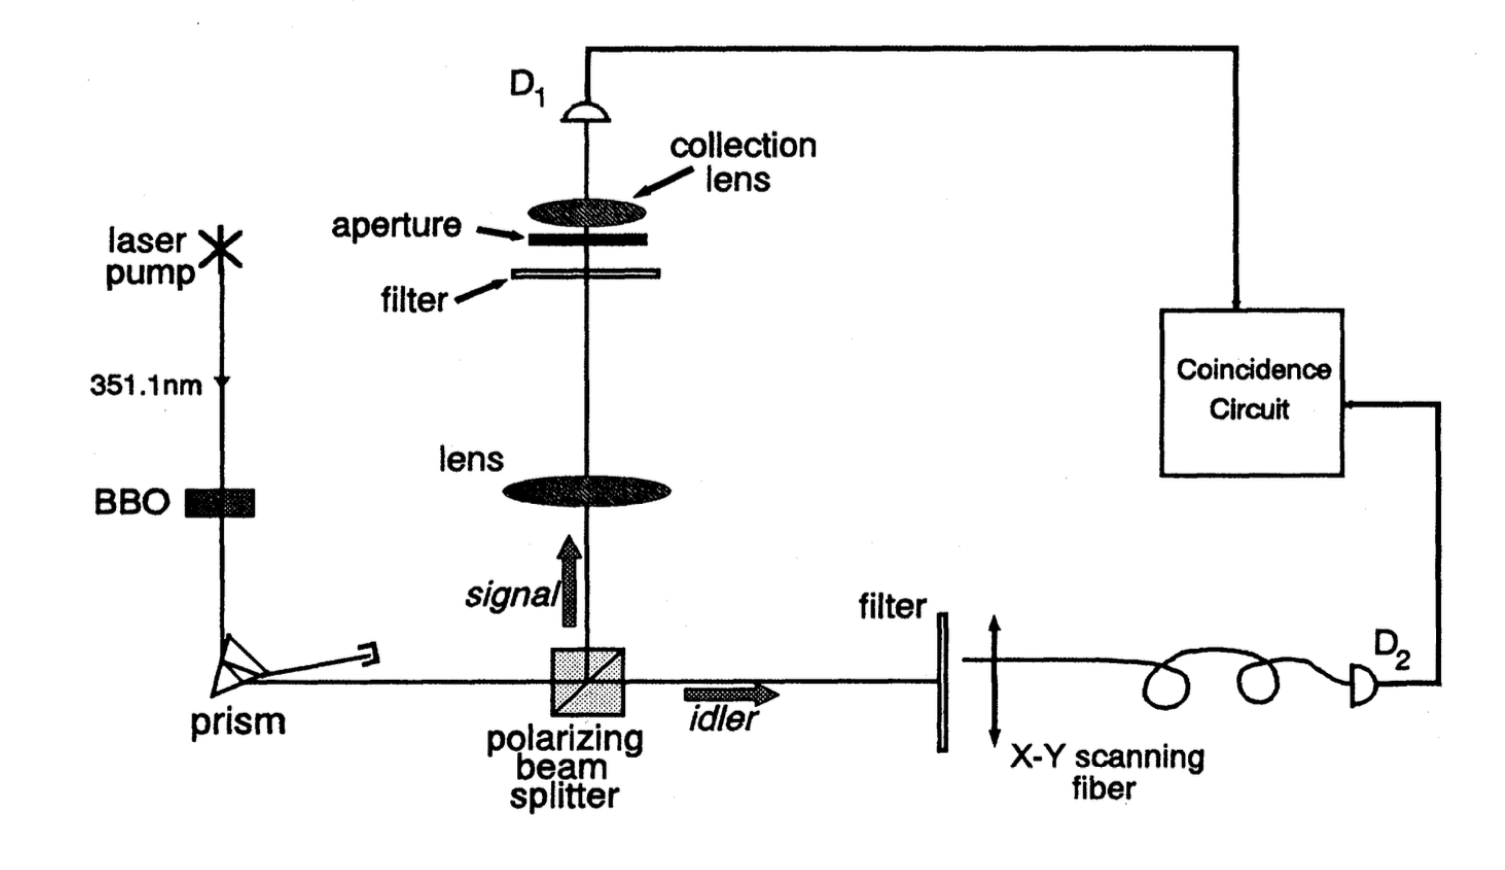
\includegraphics[width=0.5\textwidth]{Figures/pittman.png}
\caption{Schematic of the first "two-photon imaging" experimental setup, used by Pittman\cite{pittman}} 
\label{fig:pittman}
\end{figure}
A continuous wave (CW) laser is used to pump a nonlinear 
crystal to produce pairs of entangled photons. This pairs of orthogonally polarized signal and idler photons are the product
of the nonlinear optical process of spontaneous parametric down-conversion (SPDC).
The pair emerges from the crystal collinearly\footnote{The pairs emerge from the crystal nearly 
collinearly, with $\omega_s \simeq \omega_i \simeq \omega_p / 2$. where the subscript
letter stands for signal, idler and pump respectively}, it is separated by a dispersion prism, 
and then the signal and idler are sent in different directions by a polarization
beam slitting Glan-Thompson prism. 

The reflected signal beam passes through a 
convex lens with a $400mm$ focal length and illuminates an aperture\footnote{The aperture 
consisted of the letters UMBC, University of Maryland Baltimore County.}.
Before the aperture is placed a filter (Figure \ref{fig:signal}), 
this is a bandwidth spectral filters centered at the
wavelength $702.2 nm$. 
Behind the aperture is the detector package $D_1$. \\
\begin{figure}[H]
\centering
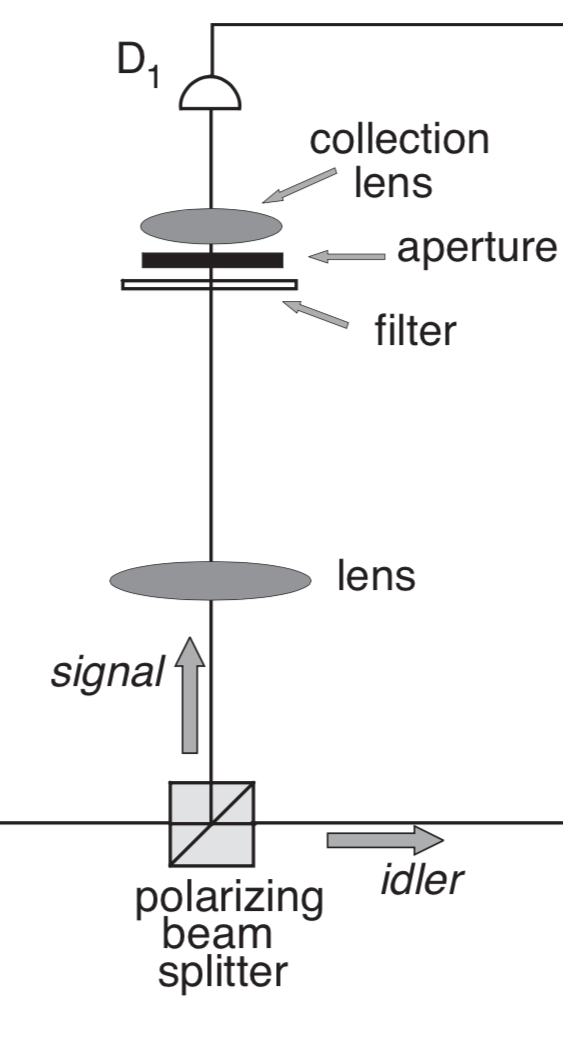
\includegraphics[width=0.24\textwidth]{Figures/signal.png}
\caption{The reflected photon, called signal} 
\label{fig:signal}
\end{figure}


The transmitted idler beam is met by detector 
package $D_2$. The input tip of the fiber is scanned in the transverse 
plane. The counts are sent to a coincidence 
counting circuit with a $1.8ns$ acceptance window.


An important fact of this experiment is the use of a lens(collection lens) in the signal beam that establishes 
an image plane with the definitive point-by-point correspondence object(mask) plane.





The Biphoton then takes a quadratic form:
\begin{equation}\label{eq:quadratic}
\tilde{\Phi}(q_s,q_i)=N exp\left[ -\frac{1}{2}x^T A x + i b^T x \right]
\end{equation}
where N is a normalization constant, $x$ is a 4-dimensional vector defined as $x = (q^x_s, q^y_s ,q^x_i,q^y_i )$, $A$ is a 4 x 4 real-valued, symmetric, positive definite matrix and b is a 4- dimensional vector. A and b are defined from the phase-matching conditions of the SPDC process. $x^T$ and $b^T$ denote the transpose of $x$ and $b$. $A$ and $b$ are functions that depend of all the relevant parameters in the experiment such as the length of the crystal L, pump waist $w_p$, creation angles inside the crystal $\varphi_n$ and the width of the spectral filter $\sigma_n$.

A way to quantify the degree of spatial correlation we shall define 'correlation parameter':
\begin{equation}
K^\lambda = \frac{C^\lambda_{si}}{\sqrt{C^\lambda_{ss}C^\lambda_{ii}}}
\end{equation}
calculated for each direction $(\lambda = x, y)$ from the covariance matrix $C^\lambda$ with elements $C^\lambda_{kj} = \langle q^\lambda_k q^\lambda_j \rangle - \langle q^\lambda_k \rangle \langle q^\lambda_j \rangle $.


\textit{Fresnel Propagator}


Fresnel Propagator: $h(r,z)=(- \frac{i}{\lambda z})e^{(i \frac{2 \pi z}{\lambda})} \Psi (r,z)$ 
with $\Psi(r,z) = e^{(i \frac{\pi}{\lambda z })r^2}$. Thin-lens transfer function $L_f (r)=\Psi(r,-f)$
 \\
\begin{equation}\label{eq:green}
G= \int d^2 r_1 \int d^2 r_0 h(r_f - r_1,f) L_f(r_1) h(r_1 - r_0,f)
\end{equation}

The propagation is done by determining the Green function\cite{green} of the optical path
by which the beam will travel. The biphoton function
in terms of transverse momenta $\Phi_1 (q_s , q_i )$ after traveling
through two arbitrary optical paths can be expressed
in terms of the corresponding Green functions and the
initial biphoton function $\Phi(q_s , q_i )$ as:

\begin{equation}
\Phi_1 (q_s , q_i )= G_s(q_s,r_1) G_i(q_i,r_2) \Phi (q_s,q_i) 
\end{equation}
\begin{equation}
\Phi_1 (r_1 , r_2 )= \int d^2 q_s d^2 q_i \Phi_1 (q_s , q_i ) 
\end{equation}

Taking advantage of the 2-F system as a Fourier-Transform to reduce the amount of calculations. Solving \ref{eq:green} over $r_0$ and $r_1$ we have:
\begin{equation}
G(q,r_f)=C e^{\frac{i \pi}{\lambda f} r_f^2} e^{\frac{i \lambda f}{4 \pi} q^2} \delta ( q - \frac{2 \pi}{\lambda f}r_f)
\end{equation}
where C is a complex constant that depends only on $\lambda = 2\pi c$ and $f$. Then we can define the Green Functions for each path:

\begin{equation}
G_1(q_s,r_1)=G(q_s,r_1) x T(r_1) 
\end{equation}
\begin{equation}
G_2(q_i,r_2)=G(q_i,r_2)
\end{equation}

Where $T(r_1)$ is the transfer function of the object.

Gathering all the previous results we can obtain $\Phi_1 (r_1 , r_2 )=C^2 T(r_1) \Phi (\frac{2 \pi}{\lambda f}r_1, \frac{2 \pi}{\lambda f}r_2)$, which describes the biphoton at the planes of the object and the scanning detector. It shows that the biphoton at the 2F plane in terms of
$r_1$ and $r_2$  has the same form as the biphoton at the
output face of the crystal with the relationship $q = \frac{2 \pi}{\lambda f} r$.
This allows to computationally simulate the biphoton at the 2-F plane by using Eq \ref{eq:quadratic} without the need to computationally simulate its propagation through the 2-F system.

We are collecting all the light that interacts with the object by the means of a bucket detector, this from the mathematical point of view leave us with: 
 $\Phi_1 (r_2) = C^2 \int d^2 r_1 T(r_1) \Phi (\frac{2 \pi}{\lambda f}r_1, \frac{2 \pi}{\lambda f}r_2)$ 
The coincidence counts that will be measured by the Detectors will be proportional to the magnitude square of the resulting biphoton function $\Phi_1 (r_2)$.
\begin{equation}
S(r_2) \propto |  \int d^2 r_1 T(r_1) \Phi (\frac{2 \pi}{\lambda f}r_1, \frac{2 \pi}{\lambda f}r_2) |^2
\end{equation}

For non-ideal forms of $\Phi (q_s,q_i)$ we have the relation between $\Phi (q) \rightarrow \Phi (r)$ for a 2F system, Hence: $\Phi(r)=\frac{1}{\sqrt{det(\Sigma)(2 \pi)^4}} e^{- \frac{1}{2} r^T \Sigma^{-1} r} e^{ibr}$ \\
$\Sigma=$


--------------------------------------------------
\subsubsection{Two-photon Imaging Using Chaotic Sources}

In principle the term "thermal radiation" should refer only to radiation coming 
from a blackbody in thermal equilibrium at some temperature T. But with this realisation of thermal radiation
we have to face some characteristics of true thermal fields. Thermal radiation is also referred as chaotic light, which
have extreme short coherence time.  \textit{expand coherence time}

Thermal sources have to be understood as incoherent light, this means that we have many photons at the beam, but the frequencies they have are 
randonly distributed. In the case of entangled light, we had a light source that generated photons that all are around a given frequency, we used a diode laser at $405nm$.


\begin{figure}[h!]
\centering
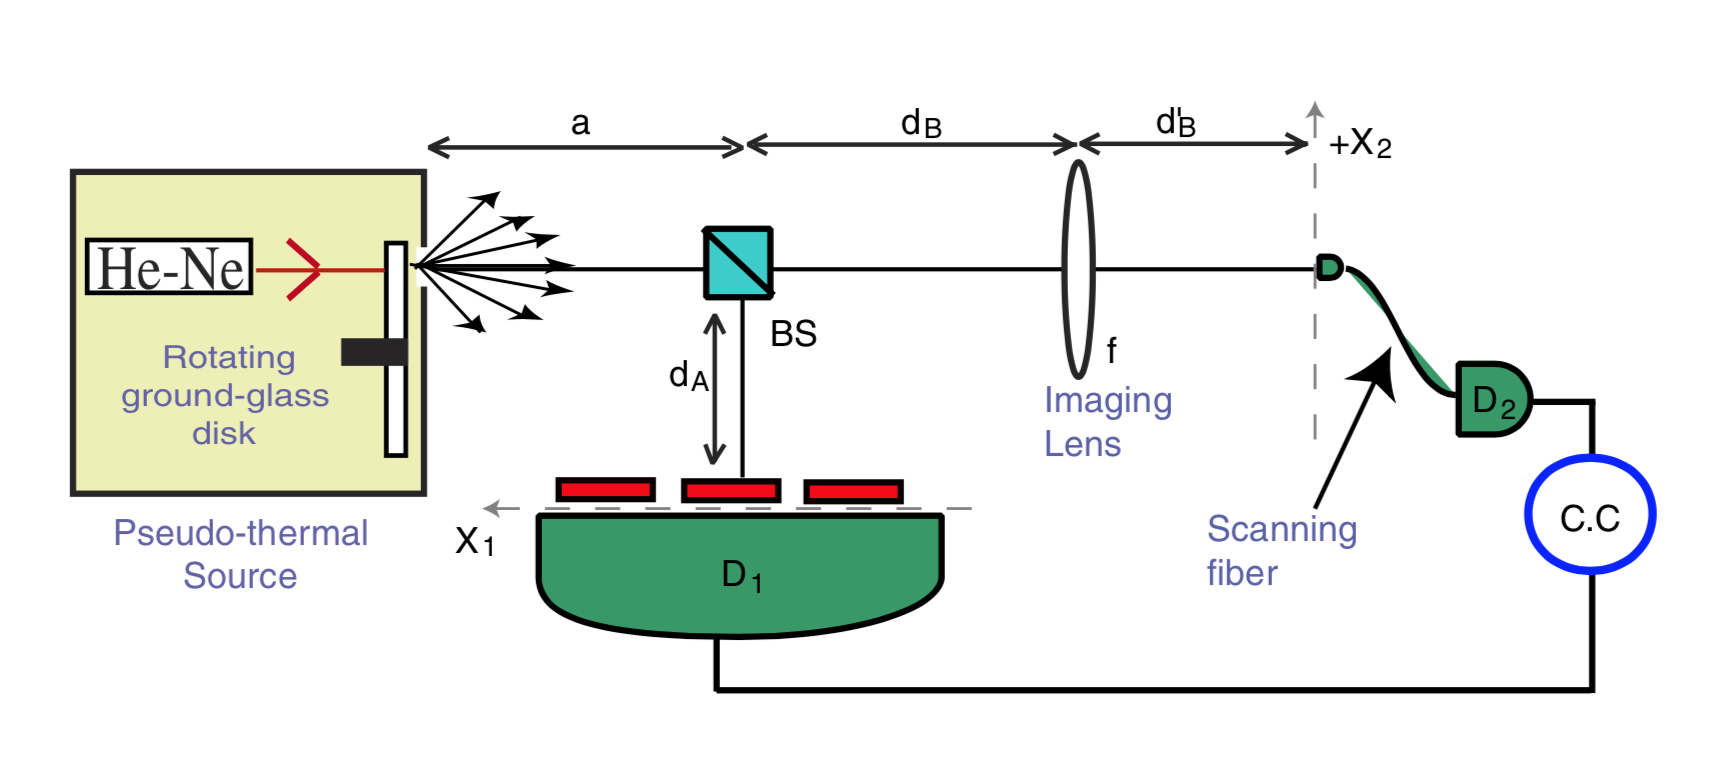
\includegraphics[width=0.6\textwidth]{Figures/thermalSetup.png}
\caption{Experimental setup for the Two-photon imaging using thermal light, taken from \cite{thermalAlejandra}} 
\label{fig:thermalSetup}
\end{figure}
The source light in Figure \ref{fig:thermalSetup} is the one developed by Martinssen and Spiller\cite{intensity}
which is the most commonly used among the pseudothermal fields.
A  coherent laser radiation is focused on a rotating ground glass disk, 
the scattered radiation is chaotic with a Gaussian spectrum.




It is possible to establish an analogy
between classical optics and entangled two-photon optics:
the two-photon probability amplitude plays in entangled
two-photon processes the same role that the complex amplitude
of the electric field plays in classical optics  \cite{thermalAlejandra}.